\begin{figure*}
  \begin{center}
    \begin{tabular}{c}
      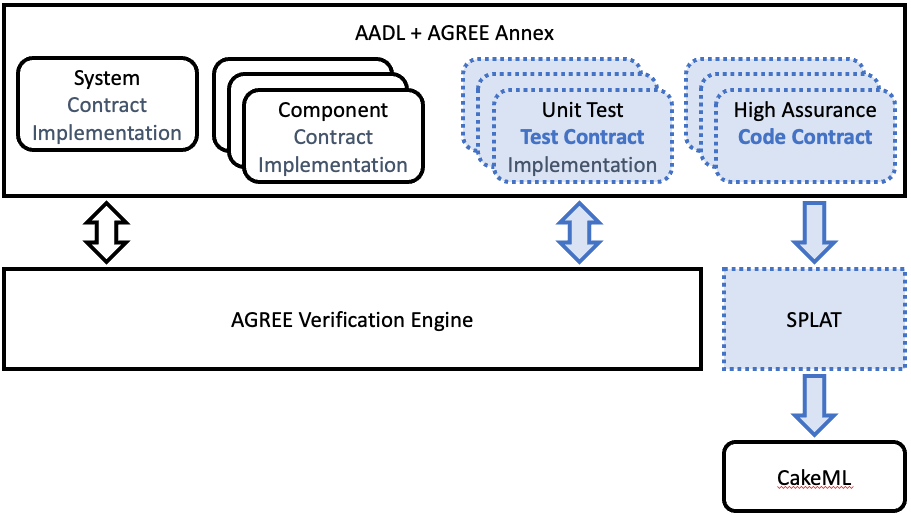
\includegraphics[scale=0.4]{flowchart.png} \\
    \end{tabular}
  \end{center}
\caption{AGREE failure certificate for initial design.}
\label{fig:example-certificate}
\end{figure*}

\begin{figure*}[h]
  \begin{center}
    \begin{tabular}{c}
      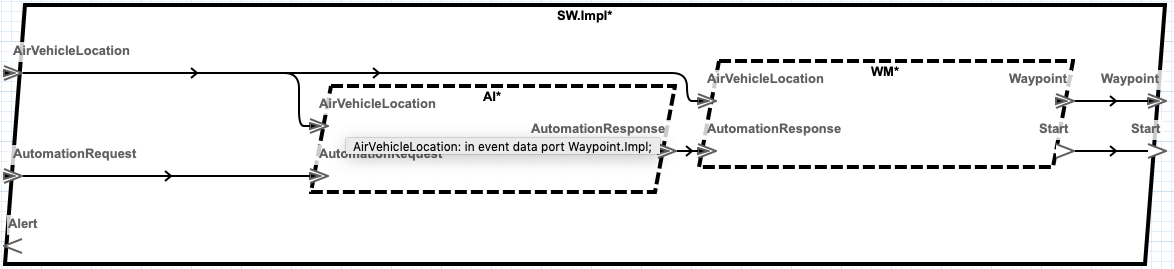
\includegraphics[scale=0.4]{example.png}
    \end{tabular}
  \end{center}
\caption{Initial design for an automated UAV route planning system.}
\label{fig:example}
\end{figure*}

\begin{figure}
  \begin{center}
    \begin{tabular}{c}
      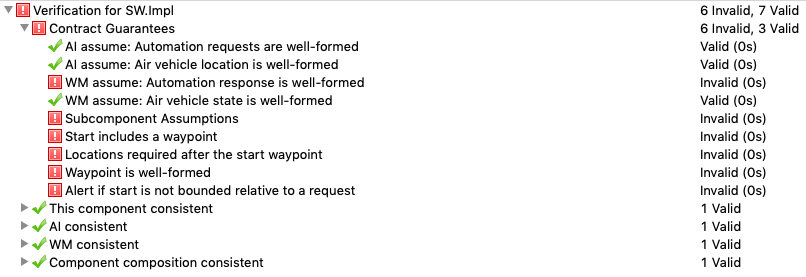
\includegraphics[scale=0.4]{example-certificate.png} \\
    \end{tabular}
  \end{center}
\caption{AGREE failure certificate for initial design.}
\label{fig:example-certificate}
\end{figure}

\egm{
  Merge the AGREE overview here into this section.
  Condense it down to just the opening two paragraphes that currently exist in the overview section.
  Walk through the first part of the example up to where AGREE fails because of Cyber Requirements.
  Introduce the new figure showing its workflow.
  Finish the example walking through the new figure. 
  Add the tests to occur before final AGREE check.
  Send to SPLAT to get verified CakeML code. 
}

We now describe a simple software system, named SW, for route planning
and automated control of a UAV. A picture of the AADL architectural
model for SW is in \figref{fig:example}. SW is loosely based on one of
the case studies in Section~\ref{sec:case-study}.  The source for the
entire model is found at \cite{repo}.

From time to time, SW receives a message on the \texttt{AutomationRequest} input,
forwarding it to a route planner (AI). The function of AI is to 
compute the flight path (a list of waypoints) for the UAV, outputting
the resulting \emph{mission command} on \texttt{AutomationResponse}.
The waypoint manager (WM) receives the mission command from AI and
starts the UAV flying the mission by putting an \emph{event} on the
\texttt{Start} output port, continuing to issue waypoints to the UAV
flight controller on the \texttt{Waypoint} port as the UAV location
updates with messages on \texttt{AirVehicleLocation}.
An event is repeatedly generated on \texttt{Alert} if there is no
mission command from a request. The AI component is third-party
software and WM is a legacy component.

%% that cannot be modified so it critically relies on
%% assumptions about its input behavior to guarantee its intended output
%% behavior.

The expected behavior of the SW system, and the components
implementing the system, is modeled with AGREE contract
specifications.  The contracts constrain input with assumptions and
state properties of output with guarantees.  AGREE performs model
checking on this assume-guarantee system to hierarchically prove that
the SW component obeys all contract obligations under all possible
finite input streams.  The AGREE analysis, contract language, and
contracts for SW are discussed in greater detail in
\secref{sec:agree} and \secref{sec:agree-semantics}.

The AGREE contracts for the initial system in \figref{fig:example},
and its implementing components, both assume and guarantee the absence
of any malicious, or unspecified, component behavior.  More precisely,
the contract for SW assumes that its inputs are \emph{well-formed} and that
there is never more than one automation request pending at a time.
Well-formed generally refers to a syntactic restriction on
data at a port. For example, a waypoint is well-formed if it falls
within bounds for latitude, longitude, and altitude.)  The guarantees
for SW ensure that
\begin{compactitem}
\item a start coincides with a new waypoint message being output;
\item a start is within one cycle of an automation request and if not, then it persistently alerts;
\item new waypoints coincide with air vehicle location updates; and
\item all outputs are well-formed.
\end{compactitem}

The contracts for the sub-components assume their inputs are
well-formed, and they guarantee their outputs are well-formed.  The AI
contract guarantees it only responds to automation requests and always
in the same cycle.  The legacy WM contract guarantees the following if
its input assumptions hold:
\begin{compactitem}
  \item it generates a start from a response from the AI and always in the same cycle;
  \item the start always coincides with a waypoint being output; and
  \item any further waypoints coincide with air vehicle location updates.
\end{compactitem}
These initial specifications pass verification, meaning that the
contract composition of the components with the system satisfies all
component input assumptions and system output guarantees.

\subsection{Detecting and addressing vulnerabilities}
A cyber-vulnerability analysis, however, identifies the potential of a
supply chain attack through the AI route planner (provided by a
third-party vendor without source code).  BriefCASE marks the
component as \emph{untrusted} after the analysis, and the contract for
AI is modified by removing all guarantees on its outputs to reflect
its untrusted status.  The AI output is now unconstrained in the
assume-guarantee reasoning of AGREE and is able to generate any value
on its output at anytime.

The output from the AGREE analysis using the untrusted AI
specification is shown in \figref{fig:example-certificate}.  The red
exclamation points designate component assumptions or system output
guarantees that do not hold, and each failure comes with a
corresponding counter-example.  The results are not unexpected given
the AI route planner's unconstrained behavior.

For example, the first violation is that the mission command on \texttt{AutomationResponse} from
the AI to the WM is no longer guaranteed to be well-formed.  The
consequence of that failing input assumption is that the WM outputs
are no longer guaranteed; they are effectively unconstrained.  These
missing output guarantees from the WM lead to the rest of the failures
in \figref{fig:example-certificate} because the WM provides the system
level outputs.

\begin{figure*}
  \begin{center}
    \begin{tabular}{c}
      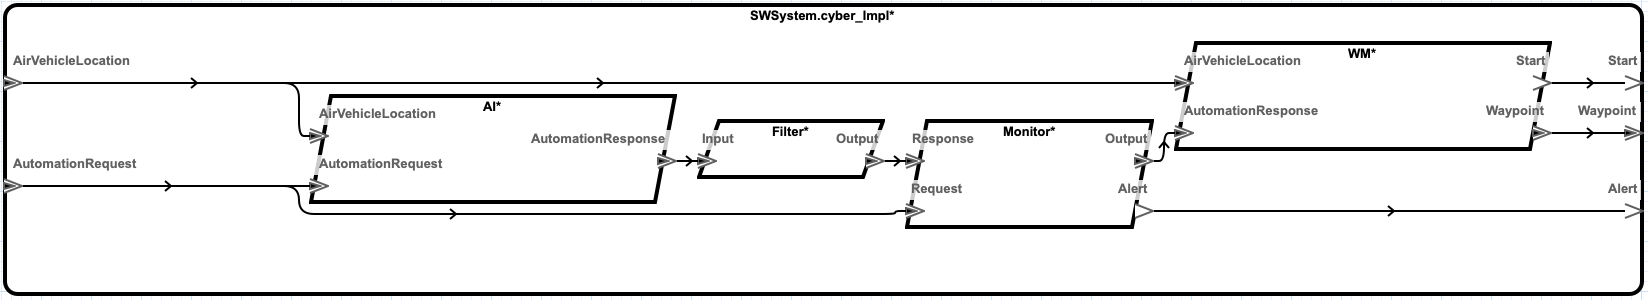
\includegraphics[scale=0.3]{hardened.png}
    \end{tabular}
  \end{center}
  \caption{Cyber-hardened design for an automated UAV route planning system}
  \label{fig:hardened}
\end{figure*}

\begin{figure}
  \begin{center}
    \begin{tabular}{c}
      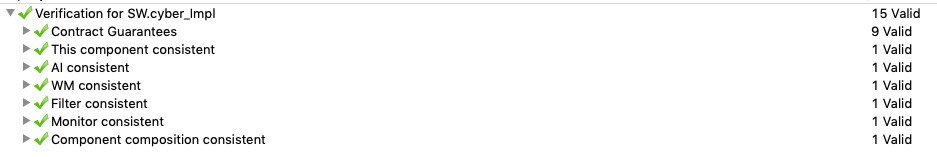
\includegraphics[scale=0.4]{hardened-certificate.png}
    \end{tabular}
  \end{center}
  \caption{AGREE verification certificate for cyber-hardened design.}
  \label{fig:hardened-certificate}
\end{figure}

The system designer now uses BriefCASE to cyber-harden SW by inserting
high-assurance components in the form of a filter and a monitor, as
shown in \figref{fig:hardened}, to isolate the AI component and prevent it from violating the WM component input assumptions.
A filter enforces an invariant over
each datum in the data stream by not forwarding input to its output if
that input violates the filter invariant.  The auto-generated AGREE
code contract specification states that only well-formed inputs are passed to the
output.  The system developer must further define the filtering
policy, but it is usually based on the existing assumptions made by
downstream components that consume the filter output.

A monitor captures a relation on input data over time and is thus able
to reason about the temporal, and other invariant, properties of that input.  A monitor raises
an alert if the specified properties are ever violated.  The
AGREE code contract for the monitor in our example states that an
automation response can only be generated in conjunction with an
automation request; and further, that response must come with the
request or in the next step after the request.  As with the filter,
the system designer provides the policy, and that policy is typically
based on existing the assumptions and guarantees of the SW system and its implementing components.
AGREE code contracts are discussed in detail in \secref{sec:code-contracts}.

The AGREE analysis of the cyber-hardened implementation is shown in
\figref{fig:hardened-certificate}. AGREE has generated high-level
evidence justifying the claim that the high-assurance components
guarantee the correct behavior of the SW implementation in the
presence of the untrusted AI route planner.  Having passed AGREE
verification, the high-assurance components are ready to be
synthesized.

\subsection{Code synthesis}
High-assurance components are automatically synthesized by SPLAT from
the AGREE code contracts to equivalent programs in the CakeML
language.
%% Too strong at the moment!
%The synthesis toolchain generates a proof that equates the
%% meaning of the AGREE specification to the behavior of the CakeML
%% program.
 In other words, for any set of input streams that meet the
 component's contract assumptions, the output streams produced from
 the synthesized CakeML code exactly match those defined by the
 high-assurance component's guarantees.  The CakeML compiler provides
 verified compilation to binaries for several different platforms,
 meaning that the resulting binaries exactly preserve the meaning of
 the original CakeML code \cite{cakeml}.

Preserving the input to output relationship of streams between the
AGREE contracts and CakeML lifts the AGREE contract verification
results to the actual deployed system.  If the contract model
verification succeeds, then the meaning of those results hold for the
deployed system.  These results, however, are only valid under
additional assumptions on the deployed system:
\begin{compactitem}
\item contracts for non-synthesized components accurately model their deployed
counterparts;
\item an appropriate schedule exists to sequence component
  execution following the dependent data-flow in the design; and
\item the communication fabric stitching components together works in harmony
  with the schedule.
\end{compactitem}
\noindent Support and automation for these aspects of the design process are
discussed in other works \cite{gearcase2020, dcrypps2019, 10.1007/978-3-030-89159-6_18, 10.1007/978-3-030-89159-6_17, sel4-2009, scheduled-agree, 9734792}.
